\section{Durchführung}
\label{sec:Durchführung}

\subsection{Aufbau}

Für die Durchführung des Versuches wird der Aufbau benutzt, der in Abbildung \ref{fig:aufbau}
dargestellt ist. 

\begin{figure}[H]
    \centering
    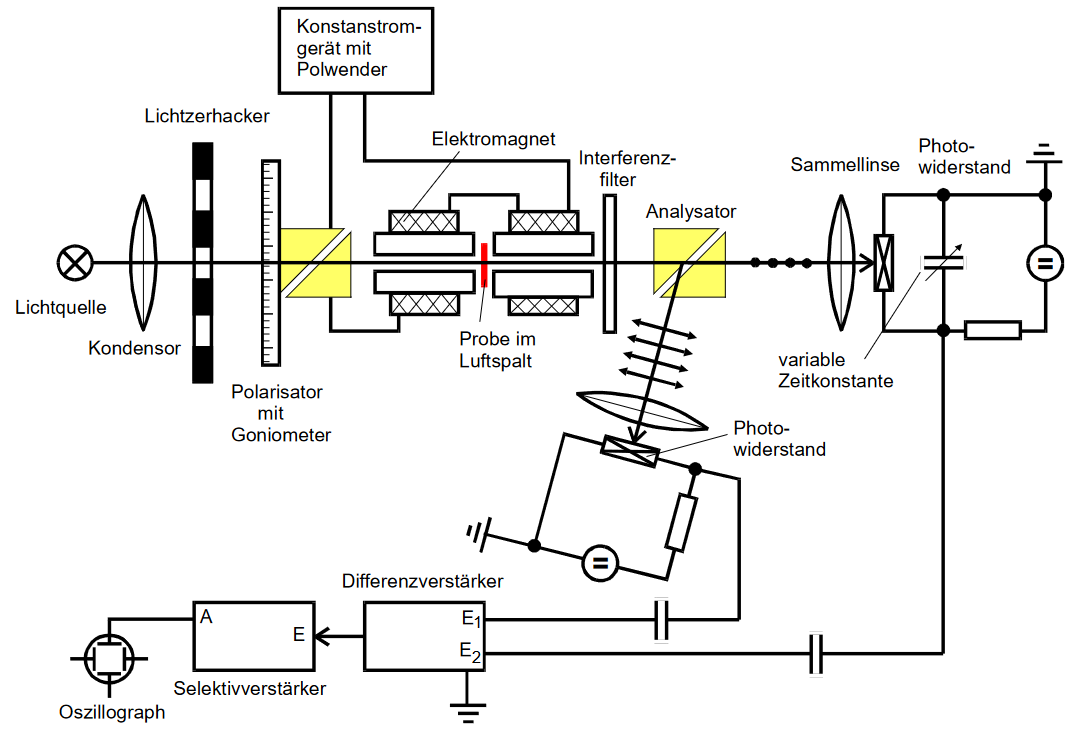
\includegraphics[width=\textwidth]{Bilder/aufbau.png}
    \caption{Aufbauskizze des Versuchs \cite{faradayeffekt}.}
    \label{fig:aufbau}
\end{figure}

\begin{figure}[H]
    \centering
    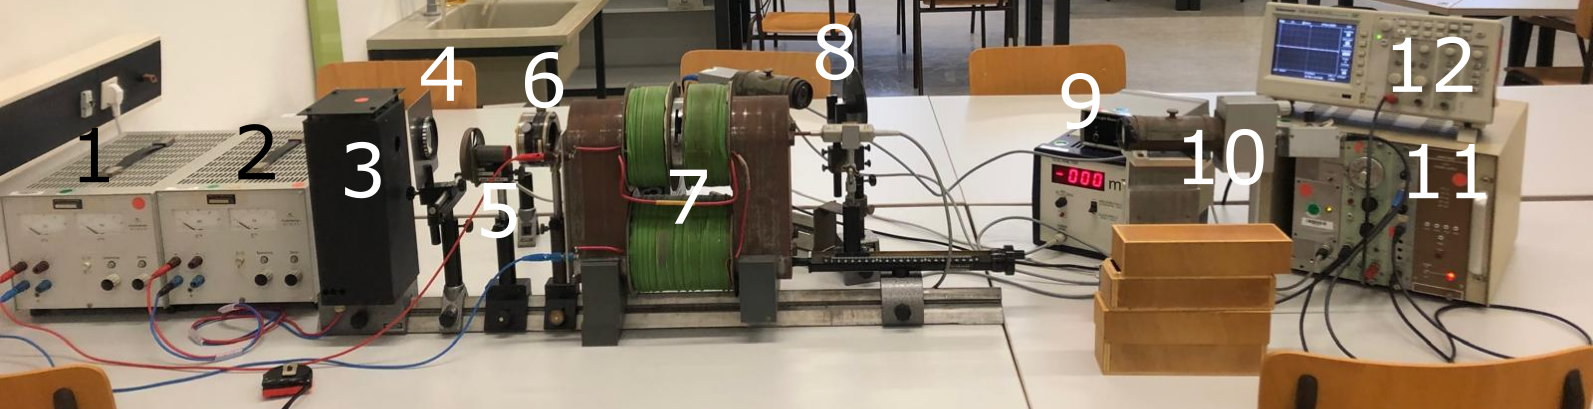
\includegraphics[width=\textwidth]{Bilder/image1.png}
    \caption{Aufbau des Versuchs. 1: Stromversorger für den Elektromagneten. 2: Stromversorger für die Halogenlampe. 3: Halogenlampe mit Gehäuse. 4: Kondensor. 5: Chopper. 6: Polarisationsfilter mit Goniometer. 7: Elektromagnet. 8, 10: Photodioden. 9: Teslameter. 11: Differenz- und Selektivverstärker. 12: Oszilloskop.}
    \label{fig:aufbau}
\end{figure}

Als Lichtquelle wird eine Halogenlampe benutzt, da diese auch im Infraroten strahlt, für das Gallium-Arsenid transparent ist. Ein Kondensor fokussiert das Licht. Ein Lichtzerhacker erzeugt aus dem kontinuerlichen
Lichtstrom Lichtpulse mit einer Frequenz von ungefähr $\qty{450}{\hertz}$. Das Magnetfeld wird mit Elektromagneten erzeugt, die bei ungefähr $\qty{20}{\volt}$ und $\qty{10}{\ampere}$ betrieben werden. Intereferenzfilter hinter
dem Magneten selektieren die Frequenzen, die detektiert werden. Ein Glan-Thompson-Prisma teilt das Licht in seine zwei Polarisationsrichtungen auf, sodass die zwei entstehenden Strahlen von Photowiderständen detektiert werden.
In einem Differenzverstärker wird der Unterschied dieser beiden Signale gemessen und ein Selektivverstärker, der auf die Frequenz des Lichtzerhackers eingestellt ist, filtert das Rauschen der Photodioden raus. Auf einem Oszillographen
kann man das entstehende Signal sehen. \\

Das Magnetfeld kann über die Stecker des Elektromagneten umgepolt werden, sodass es einemal in Lichtausbreitungsrichtung gerichtet ist und einmal entgegen. Das ermöglicht die Messung von zwei Winkeln der Polarisation,
deren Differenz am Ende ebenfalls ausgewertet werden kann, um ein genaueres Ergebnis zu erhalten. \\

Der Versuch wäre ebenso mit nur einem Detektor ausführbar, aber entsprechend ungenauer.\\

\subsection{Messung}

Für die korrekte Durchführung werden die Photowiderstände so ausgerichtet, dass die Teilstrahlen auf eben diese treffen. \\
Zu Beginn wird das Magnetfeld mit einer Hallsonde an verschiedenen Stellen innerhalb der Spule vermessen. \\

Eine Gallium-Arsenid-Kristall wird in das Feld eingeführt und mit polarisiertem Licht bestraht. Ein Interferenzfilter, der eine bestimmte Wellenlänge des Lichtes durchlässt, wird hinter den Kristall in den Lichtstrahl gestellt.
Die Polarisation wird so gewählt, dass das Signal auf dem Oszilloskop minimal wird. Zu der entsprechenden Wellenlänge wird der eingestellte Winkel gemessen. Dies wird für acht weitere Wellenlängen wiederholt. Anschließend wird das Magnetfeld
umgepolt und die Wiederholt der neun Wellenlängen erneut durchgeführt. Für eine Wellenlänge ergibt sich der gedrehte Winkel in einer Probe der Länge $L$ dann nach den zwei Messungen zu
\begin{equation}
<<<<<<< HEAD
    \theta = \frac{1}{2}(\theta_1 - \theta_2)
||||||| 05b9994
    \theta_\text{frei} = \frac{1}{2}(\theta_1 - \theta_2).
=======
    \theta_\text{frei} = \frac{1}{L} \frac{1}{2}(\theta_1 - \theta_2).
>>>>>>> 488e4e5413ead7ea746f355c1424b3fbb286a0b0
    \label{eq:theta}
\end{equation}
und der auf die Länge $L$ normierte Drehwinkel freier Elektronen Ist
\begin{equation}
    \frac{\theta_\text{frei}}{L} = \frac{\theta_\text{dotiert}}{L_\text{dotiert}} - \frac{\theta_\text{rein}}{L_\text{rein}},
    \label{eq:thetafrei}
\end{equation}

Es werden insgesamt drei Gallium-Arsenid-Kristalle vermessen, einer ohne Dopants und zwei mit verschieden hohen Konzentrationen. \\

